The main requirement of the FAR-EDGE CPS Data Model is to provide full support to the \textit{Open API for Virtualization}. 
In othe words, the data model has to be designed with the goal of : 
\begin{enumerate}
\item providing tools to fully describe simulation models to be imported and executed in one of the two simulators that FAR-EDGE supports
\item allowing the user to define complex synchronization processes to be carried out by the Real-to-Digital Synchronization (R2DS) Component and the \textit{Edge Analytics Engine}. 
\end{enumerate}

The Real-to-Digital Synchronization (R2DS) can be defined as the process of continuously updating CPS models stored in the \textit{Model Repository}, following the evolution of the shop floor. 
Having up-to-date models is especially important in simulation. 
In fact, machines along their life cycle are subject to aging, straining, and reconfiguration processes, which might affect their behavior and performance; in this case the simulation outcomes to drift apart substantially from reality and, therefore, result useless. 
In order to be able to make informed decisions based on reliable simulation models, it is of paramount importance to detect changes in the model automatically and continuously, and to adapt parameters and scenarios accordingly. 

The core of the R2DS grounds in the processing of data gathered at shop floor level. 
It is worth noticing that this is a general approach, based on data processing, which enables not only the tracking of CPS models parameters but it also unlocks scenarios where, for instance, digital twins can be enriched with inferred pieces of information that cannot be directly measured from the field. 
For illustration purposes, let's imagine the case in which a digital twin is extended with the results of a machine learning algorithm for predictive maintenance~\cite{daily2017predictive}. This information, in turn, could be used from the simulation to schedule the most suitable time to perform the maintenance of the real machine.  
Having based the synchronization process on a general-purpose data analytics engine has the non-secondary benefit to leave the overall architecture independent from the simulation domain. The other side of the coin is that, with this approach, the definition of the synchronization procedure must be implemented as part of the data model. 
This is because each digital twin might require a different data processing (a.k.a. \textit{Synchronization Model} - SM) to be synchronized with its real counterpart. 

Synchronization Models describe the way data from the field must be processed to update the model attributes or to estimate indirect values and create new attributes. 
A synchronization model contains an algorithmic description of how to process data from machine sensors at shop floor level in order to generate updates that continuously serve to keep the digital twin digital in sync with the related CPS. 
This description can therefore be instantiated in different ways depending on the technological choices that underlie the implementation of the platform. 
The solution adopted in the project is to implement the synchronization model in the form of a simulation asset, that is a binary file containing executable code and to associate it with the representation of a CPS within the data model. The synchronization model, therefore, in order to perform its duty, must be compiled, installed and managed within a suitable execution environment, which can provide through an API the abstractions necessary to process data coming from the production environment in a distributed way.  


Specific components will be in charge of managing the life cycle of Synchronization Models, which includes: 
\begin{itemize}
\item \textbf{checking the execution schedule}: depending on the synchronization scenario the SM can be continuously executed against streams of field data (if the CPS is reachable and producing data), or it is scheduled to run periodically, say for instance, once a day over historical data. 
\item \textbf{model fetching}: the SM persisted in a suitable database is looked up and retrieved. 
\item \textbf{execution}: the SM is run exploiting FAR-EDGE Open API for Analytics and Synchronization Services
\item \textbf{application of the updates}: the SM generates attribute values for the related digital twin. These values are used to update the digital twin, which the model refers to.
\item \textbf{model dismissal}: once the dismissal condition is verified as, for instance, the CPS is not connected or the synchronization process ended the SM is dismissed and the \textit{Synchronization Services} sub-system is notified.
\end{itemize}

Figure~\ref{fig:r2ds} describes graphically a reference scenario where a CPS, registered and connected to the FAR-EDGE platform, is switched on and a data flow is spawned via the \textit{Data Routing and Preprocessing Component} of the architecture. 
The R2DS Component is notified and, if a SM is associated with the CPS digital twin in the model repository, it will be retrieved and executed on the Synchronization Services, which in turn rely on the Edge Analytics Engine. 
In this scenario, the SM will process the input data flow and generate in output a new one, containing for each time interval the updates to be applied to the corresponding digital twin. 
The R2DS component is in charge of performing the model update process. 
It is worth restating at this point that the algorithm implemented within a SM it is not constrained to the generation of attribute updates for digital twins, but it is general. In this way, for instance, the same infrastructure and the overall process can be used to enrich the CPS definition with new pieces of information. 

\begin{figure}
	\centering
	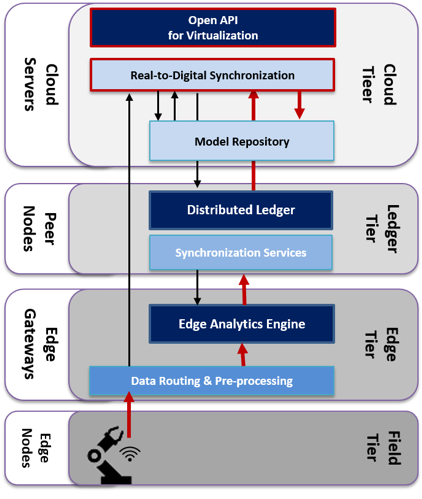
\includegraphics[width=0.6\linewidth]{images/R2DS}
	\caption{Synchronization process in the scenario of data stream processing}
	\label{fig:r2ds}
\end{figure}


